\chapter{Introduction}
\label{ch:intro}

\section{Obesity}
\label{sec:obesity}

Obesity has been a major global problem for more than a decade, associated with many noncommunicable diseases such as diabetes, cardiovascular diseases and certain types of cancers \citep{WHO2014}.
In fact, the risk of comorbidities increases with an increase in \gls{bmi}, where the risk becomes severe as the \gls{bmi} level approaches the obese category \citep{WHO2000}.
The number of overweight and obese people, in both adults and children, has risen in every country of the world and the trend will likely to continue in the future.
It is estimated to account for 3.4 million deaths per year and 93.6 million \glspl{daly} in 2010, obesity is a serious disease that continues to grow in our society \citep{Lim2012}.

\subsection{Definition of obesity}
\label{sub:definition_of_obesity}

Obesity is defined as an abnormal or excessive fat accumulation that may impair the health of an individual \citep{Garrow1988}.
One common and widely used approach to categorise obesity is to measure the \gls{bmi} of the individual.
\gls{bmi} is a measurement based on the weight-to-height ratio of an individual.
It is often used by clinicians and epidemiologists to classify adults into underweight, normal weight, overweight, or obese categories.
The unit of \gls{bmi} is defined as the weight in kilograms per square of the height in metres (kg/m$^2$).

The \gls{who} (2014) categorise overweight and obese adults  with a \gls{bmi} of  $\geq$ 25 kg/m$^2$ and $\geq$ 30 kg/m$^2$ respectively.
For children under the age of 5, overweight and obesity is categorised as a  weight-for-height ratio greater than 2 standard deviation and 3 standard deviation above the \gls{who} Child Growth Standards median respectively.
For children aged between 5 to 19 years, overweight and obesity is defined as \gls{bmi}-for-age greater than 1 standard deviation and 2 standard deviation above the \gls{who} Growth Reference Standards median respectively.

However, the use of \gls{bmi} as an accurate measure of body fat composition and/or representation of the metabolic state of an individual remains controversial.
In fact, many studies have suggested that the use of other measurements, such as waist-to-height and waist-to-hip ratios, to classify the patients into different categories, as these measurements were better predictors of the diseases related to obesity than \gls{bmi} \citep{Dalton2003,Gelber2008,Lee2008}.
With that said, \gls{bmi} is still widely used due to the ease of data collection compared to other measurements.
As a result, most of the publicly available clinical data has height and weight data of the patients from which the \gls{bmi} can be calculated.

\subsection{Prevalence of obesity}
\label{sub:prevalence_of_obesity}

From the latest global status report on noncommunicable diseases by the \citet{WHO2014}:
\begin{quote}
	\textit{
		``In 2014, 39\% of adults aged 18 years and older (38\% of men and 40\% of women) were overweight.
		The worldwide prevalence of obesity nearly doubled between 1980 and 2014.
		In 2014, 11\% of men and 15\% of women worldwide were obese.
		Thus, more than half a billion adults worldwide are classed as obese.''
	}
\end{quote}

\noindent
Approximately 1 in every 14 people in the world were classed as obese in 2014; therefore, 1 in every 14 people around the world were also at severe health risks associated with obese people.
The highest prevalence of overweight and obesity was in the American regions, where 61\% and 27\% of the population were overweight and obese respectively \citep{WHO2014}.
It was also noted in the report that women were more likely to be obese than men, and that the prevalence of overweight and obesity increased as the income level of the countries increased \citep{WHO2014}.

In addition to this, the worldwide prevalence of childhood obesity has been increasing steadily since 2000 \citep{WHO2014}.
The prevalence of overweight children in those under 5 was estimated to rise from 6.3\% in 2013 to 11\% by 2025 if the current trend continued \citep{WHO2014}.
The current prevalence of obesity in the younger population poses an even greater risk to the health of the population in the future than the current prevalence of obesity in the adult population.

In \gls{nz}, obesity is a serious problem as approximately one third (31.6\%) of adults in \gls{nz} were classified as obese in 2015/2016 \citep{Health2016}.
The Pacific and M\=aori populations were affected the most, where 67\% and 47\% of the adults, respectively, were obese \citep{Health2016}.
\gls{nz} not only has a high prevalence of obesity compared to many other countries, but also has a unique health problem that affects Pacific and M\=aori populations disproportionately than the rest of the \gls{nz} population.

\subsection{Physiological mechanism of obesity}
\label{sub:physiological_mechanism_of_obesity}

Obesity is caused by continuous intake of food without expending all of the energy gained from the food.
The key to the problem is the control of food intake and energy expenditure, and how they are regulated in the body.
The role of the hypothalamus is central to the control of satiety and many of the mutations that cause obesity affects the satiety signals to and/or from hypothalamus.
The hypothalamus receives both neuronal and hormonal inputs from the body and propagates the signal to the downstream neurons which ultimately affects the food intake of the individual \citep{Bell2005, Spiegelman2001}.

There are two types of neurons in the arcuate nucleus (located in the hypothalamus): orexogenic and anorexogenic neurons.
Orexogenic neurons are responsible for the promotion of food intake and reducing energy expenditure, whereas the anorexogenic neurons have the opposite effect \citep{Barsh2002}.
When stimulated by, for example, endocrine signals, these two different types of neurons act on the downstream neurons to promote or reduce food intake and energy expenditure.

Leptin-melanocortin pathway is the main pathway in which the level of satiety is controlled and regulated \citep{Spiegelman2001}.
In this pathway, both the orexogenic and anorexogenic neurons (located in the arcuate nucleus of the hypothalamus) have crucial roles in controlling the satiety of the individual, and therefore their eating behaviour \citep{Barsh2002,Bell2005}.
When a satiety-controlling hormone such as leptin reaches the arcuate nucleus region of the hypothalamus, it can stimulate or inhibit orexogenic, anorexogenic, or both orexogenic and anorexogenic neurons.
Depending on which neurons are stimulated or inhibited, the hormone will ultimately alter the satiety level of the individual.

Though there are many hormones that regulate satiety, only leptin and insulin will be covered here.
Leptin is a hormone that signals satiety and reduces food intake, and is secreted mainly by the white adipose tissue \citep{Moustafa2013,Zhang1994}.
The circulating concentration of leptin in the body is proportional to the body fat stores \citep{Barsh2002, Moustafa2013}.
Leptin signals through the \gls{jak}/\gls{stat} pathway via the long form of the leptin receptor that is present in high expression in the hypothalamus \citep{Ghilardi1996,Lee1996}.
Depending on the type of neurons the leptin receptor is expressed on, leptin stimulates or inhibits these neurons and ultimately produces an anorexogenic signal to the downstream effector neurons \citep{Bell2005}.

Insulin, perhaps the most well-known hormone for its role in glucose homeostasis, also has an important role in satiety and food intake regulation.
In brief terms, when insulin binds to the insulin receptor, \gls{irs} protein family is recruited and phosphorylated by the  intrinsic tyrosine kinase activity of the insulin receptor \citep{Saltiel2002}.
The phosphorylated \gls{irs} protein then activates \gls{pi3k}, which in turn activates its downstream targets, causing a rapid signal cascade through the cell \citep{Saltiel2002}.

The exact role of insulin in the satiety control was not particularly clear even though there was evidence of increased food intake with neuron-specific deletion of insulin receptor \citep{Barsh2002,Bruning2000}.
The fact that the insulin level, like leptin, was proportional to the fat mass also suggested the role of insulin in satiety and body weight control \citep{Barsh2002, Bruning2000, Woods1979}.
This was perhaps due to the fact that leptin and insulin used two different signalling pathways in the cell: leptin used the \gls{jak}/\gls{stat} signalling pathway, whereas insulin used the \gls{pi3k} pathway for signalling \citep{Ghilardi1996}.
However, leptin, and subsequently insulin, was shown to activate ATP-dep\-endent K$^+$ channel in glucose-responsive neurons in the hypothalamus \citep{Spanswick1997, Spanswick2000}.
The activation of the K$^+$ channel provided evidence for the two pathways to act similarly on the cell, at least for an acute response.
This suggests a convergence in the pathway response by the two hormones, and therefore their role in satiety control.

Satiety control is crucial in order to manage  and maintain the body weight in a healthy state.
As described above, there are many components that regulate satiety.
Disruption of any part of the satiety controlling pathway can encourage the development of obesity.

\subsection{Factors that affect the prevalence of obesity}
\label{sub:factors_that_affect_the_prevalence_of_obesity}

\subsubsection{Individual-level (micro-level) factors}
\label{ssub:Individual-level_(micro-level)_factors}

There is much evidence of obesity being caused by individual-level genetic factors that make some individuals more predisposed to obesity than others.
Generally speaking, there are two classes of genetically-driven obesity: monogenic obesity and polygenic obesity \citep{Moustafa2013}.

Monogenic obesity is where a single mutation in one of the genes that is directly involved in the satiety controlling pathway causes severe obesity in that individual.
Since these mutations are usually directly related to the key constituents in the pathway mentioned earlier (\cref{sub:physiological_mechanism_of_obesity}), the resulting phenotype from the mutation causes severe early-onset obesity.
However, although these mutations cause a devastating effect on those who carry the mutation, these mutations occur very rarely in the population.

An example of a mutation that causes severe early-onset obesity is a mutation in the leptin gene.
\citet{Montague1997} found a single nucleotide deletion mutation at position 133 of the leptin gene in children with early-onset obesity.
They further showed that the mutation caused a frameshift mutation in the protein, resulting in an inactive form of leptin that was not able to be secreted \citep{Montague1997}.
As a result, children with this mutation were constantly hungry due to the lack of anorexogenic signals and became obese at a very early stage of their lives.

Polygenic obesity is where a combination of variants in multiple genes or multiple regions of the genome (together with the effect from the environmental factors) causes obesity in the individual \citep{Moustafa2013}.
Unlike in monogenic obesity, where a single mutation in a gene causes severe obesity, the variants in some of the genes or genomic regions involved in polygenic obesity have little effect on the obesity status of the individual by itself.
However, in combination with many other variants and together with environmental factors, it has a serious obesogenic effect on the individual.

There have been many studies that have investigated the association of genes and/or genomic regions with obesity.
Of those, many of the \glspl{gwas} published in 2007 showed strong evidence of the \gls{fto} gene with \gls{bmi} and obesity  \citep{Dina2007,Frayling2007,Gerken2007,Scuteri2007}.
Until these studies came out, there has been no common genes or genomic regions found to be associated with obesity that was reproducible and reliable \citep{Frayling2007}.
Thus, these studies were the first evidence of common variants that contributed to the polygenic obesity phenotype in the population.

These individual-level genetic factors contribute to the overall increase in the proportion of the population that are obese.
However, it is likely that the environmental factors are the most significant contributor to the current global obesity epidemic \citep{Malik2013}.

\subsubsection{Population-level (macro-level) factors}
\label{ssub:Population-level_(macro-level)_factors}

It is clear that the individual-level factors cannot be accounted for the global epidemic of obesity that the world currently observes.
For this reason, obesity is thought to be caused mainly by the environmental factors that act on a population-level.
The first key factor that contributes to the global rise in the proportion of the population that is obese is the availability and abundance of certain foods in the country.
With the help from government free trade policies, food and other goods have become easier to trade between countries, helping the economic growth of many countries around the world \citep{Kearney2010}.
This has led to a greater abundance of food in general, a greater number of food choices and a change in the overall nutritional status of countries \citep{Malik2013}.
This shift in food choice and availability (and the economic benefit associated with the trade) had a positive impact on countries, but the growth in the food market also resulted in the population-wide rise in obesity.

As an example, in the \gls{usa}, the cost of corn and soy are low due to the fact that they are the raw ingredients for most processed food and beverages, such as high fructose corn syrups used to sweeten many soft drinks in the \gls{usa} \citep{Malik2013}.
Moreover, corn and soy are also the main food for livestock, which results in lower price for meat \citep{Malik2013}.
On the other hand, the prices of fruits and vegetables remain expensive due to the lack of support by the government to lower the cost associated with the production \citep{Malik2013}.
As a result, more people are inclined to consume food that are cheap, have little nutritional value and high in energy, than food that are expensive, nutritional and healthy alternatives.
Thus, the population is more likely to become obese by making poor food choice.

The second factor to consider is the behavioural changes led by urbanisation.
As more people take up urban lifestyle, they are exposed to new environments with a better range of food selection, as well as technological and mechanical advancement in transport and other daily chores that may not be available in rural areas.
Although urbanisation has many advantages, such as access to developed health care systems, education and advanced technologies, the lifestyle change also imposes negative health behaviour that ultimately can lead to positive energy balance and obesity \citep{Malik2013}.
Lack of physical activity is one of the obvious components linked with urbanisation.
In many urban cities, the recommended level of physical exercise is often difficult to achieve and maintain due to the shift towards sedentary behaviours that are encouraged by developed transport systems, automated household chores and indoor entertainment \citep{Malik2013}.

The last factor to be mentioned here is the income and socioeconomic status of the population.
As the average income increases, more people are able to buy food and are likely to take up a sedentary lifestyle.
From this, one would expect the high-income group to have the largest impact from obesity, but on the contrary, the biggest impact from obesity is seen in the low- and middle-income groups \citep{Malik2013}.
Access to a developed health care system will allow weight maintenance, but this is likely to be of most benefit to high-income groups.
The reason for this is the cost associated with a visit to the health care system, as high-income groups are more likely to make a consistent and periodic visit than a low- or middle-income groups \citep{Malik2013}.

So, for the low- and middle-income groups, the rise in the average income in these groups allows people to have access to food and activities that promotes sedentary behaviours, but the limited access to the health care system, education and recreational activities (that promote physical activity) ultimately leads to positive energy balance \citep{Malik2013}.
In contrast, the high-income group of the population have better access to facilities that promote weight maintenance, thus have less of an impact compared with the low- and middle-income groups of the population.
All of these population-level environmental factors in synergy with the individual-level genetic factors have contributed to the global epidemic of obesity.

\section{Cancer}
\label{sec:cancer}

\begin{quote}
	\textit{
	``Cancer is a generic term for a large group of diseases that can affect any part of the body \ldots{}
	One defining feature of cancer is the rapid creation of abnormal cells that grow beyond their usual boundaries, and which can then invade adjoining parts of the body and spread to other organs \ldots{}
	referred to as metastasizing.
	Metastases are the major cause of death from cancer.''
	\citep{WHO2016}
	}
\end{quote}

\subsection{Prevalence and mortality of cancer}
\label{sub:prevalence_and_mortality_of_cancer}

Cancer is considered as one of the leading causes of deaths around the world, accounting for 8.2 million deaths in 2012 \citep{WHO2014}.
More than half of cancer deaths are caused by lung, breast, colorectal, stomach and liver cancers \citep{WHO2014}.
The leading cause of cancer deaths in high-income countries is lung cancer in both men and women, then colorectal cancer and breast cancer for men and women, respectively \citep{WHO2014}.
Although the levels of mortality vary among different countries, cervical, liver and stomach cancers make up a large proportion of cancer deaths among low- and middle-income countries \citep{WHO2014}.

\citet{Bray2013} estimated the global prevalence of cancer in the adult population in 2008.
Since there was no clear definition for cancer prevalence, \citet{Bray2013} used \gls{ldp} as an estimate for cancer prevalence, and measured the incidence of cancer during the period between 2004 and 2008 (5 years).
From these estimates, Eastern Asia had the greatest 5-year prevalence of cancer, with approximately 7 million people with cancer in 2008, followed by North America and Western Europe with approximately 4.7 and 3 million people with cancer \citep{Bray2013}.
When the population of these regions was taken into account and the proportion of cancer prevalence calculated, Western Europe had the highest prevalence proportion of 1.9\%, followed closely by Australia/New Zealand with 1.82\% and North America with 1.7\% \citep{Bray2013}.

Looking at the prevalence of cancer by specific types, breast cancer was the most prevalent type of cancer with 5.2 million cases in 2008 \citep{Bray2013}.
Colorectal and prostate cancers were the second and third most prevalent cancer types, with approximately 3.2 million cases \citep{Bray2013}.
\citet{Bray2013} noted that female-specific cancer types were the most prevalent types of cancer in 75\% of countries in the world.
Furthermore, the prevalence of breast, cervix or prostate cancer is the highest in almost 95\% of countries \citep{Bray2013}.
Although these estimates provide a relatively crude measure of cancer prevalence, \citet{Bray2013} provided a useful overview of the prevalence of cancer  around the world.

In \gls{nz}, the most common cancer types diagnosed for males are prostate, colorectal, melanoma, lung and non-Hodgkin lymphoma, which all together accounted for 65\% of newly registered cancers in males in 2013 \citep{Health2016b}.
For females, breast (which accounted for 28.3\% of all new female cancer cases), colorectal, melanoma, lung and uterine cancers were the most common cancer types diagnosed in 2013 \citep{Health2016b}.
The cancer registration rates were higher in females aged 25-54 years than males of the same age group, but the registration rates were significantly higher in males for people who were 60 years or older \citep{Health2016b}.
Like with obesity, there is a significant difference in the cancer registration rates between M\=aori and non-M\=aori.
The rates were 1.2 and 1.4 times greater in the M\=aori population compared to the non-M\=aori population for males and females, respectively \citep{Health2016b}.
Again, this difference between the M\=aori and non-M\=aori is unique to \gls{nz}, and improved understanding of the underlying problem is essential for better treatment plans and outcomes for M\=aori.

The total number of deaths by non-communicable diseases (including cancer) is predicted to increase, reaching 52 million deaths by 2030 \citep{WHO2014}.
With the prevalence of cancer at such high levels around the world, and with cancer mortality increasing in the future, cancer is a serious challenge that the world has to face.

\subsection{Mechanisms of cancer development}
\label{sub:mechanisms_of_cancer_development}

It is now commonly understood that cancers are caused by dysregulation of various molecular mechanisms or pathways that allow tumour cells to proliferate, survive and migrate.
By taking advantage of these pathways, cancer cells are able to grow and eventually metastasise to other parts of the body.
The environment in which the tumours arise can also be an important factor for their evolution and growth.

\subsubsection{Hallmarks of Cancer}
\label{subsubsec:cancerhallmarks}

Extensive research in cancer biology has uncovered many pathways and regulatory mechanisms involved in cancer.
With more than 100 distinct types and subtypes of cancers, each with its own distinct development mechanisms, it became difficult to focus on the overarching mechanisms of cancer development \citep{Hanahan2000}.
To resolve this, \citet{Hanahan2000} proposed ``six essential alterations'' that cancer cells usually take advantage of during development and progression.
These six key mechanisms were coined as being ``The Hallmarks of Cancer'', and have been used extensively by many researchers as their guide to target their research in specific areas of cancer biology.

Ten years after the first review where the concept of Hallmarks of Cancer was proposed, Hanahan and Weinberg revisited these hallmarks and added four more on top of the six hallmarks presented in 2000 \citep{Hanahan2011}.
The ten Hallmarks of Cancer are: sustaining proliferative signalling, evading growth suppressors, enabling replicative immortality, activating invasion and metastasis, inducing angiogenesis, resisting cell death, avoiding immune destruction, tumour-promoting inflammation, genome instability and mutation, and deregulating cellular energetics (\cref{fig:hallmarks}).
Each of these hallmarks will be described briefly to provide an overview of the significance of these mechanisms in tumour biology.

\begin{figure}[htb!]
	\centering
	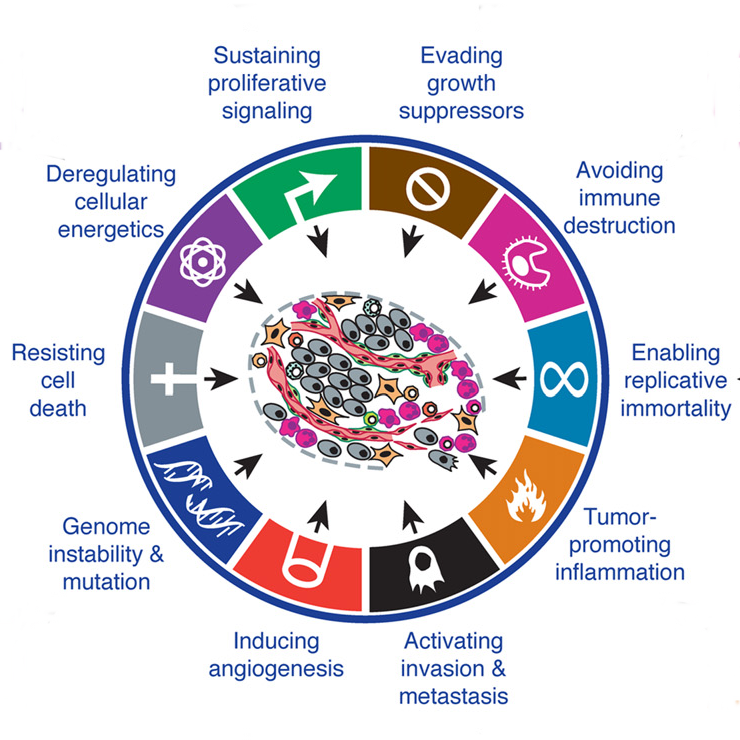
\includegraphics[width=0.8\linewidth]{intro/hallmarks}
	\caption[Hallmarks of Cancer]{Hallmarks of Cancer. The ten Hallmarks of Cancer as proposed by Hanahan and Weinberg in 2011. (Figure adapted from \citet{Hanahan2011})}
	\label{fig:hallmarks}
\end{figure}

\paragraph{Sustaining proliferative signalling}

\noindent
Cancer is a disease of uncontrolled cell proliferation and division.
Normal cells cannot proliferate without any external mitogenic growth signals, but cancer cells are able to deregulate these signals to maintain a steady proliferative signal \citep{Hanahan2011}.

There are many ways in which cancer cells can maintain this signal.
Firstly, cancer cells can acquire the ability to produce growth factors and express the corresponding receptor, creating a positive feedback mechanism that continuously stimulates the cells to proliferate \citep{Hanahan2000}.
Secondly, they can express more receptors for a given growth signal, and thus become ``hyperresponsive'' to the signal \citep{Hanahan2000,Hanahan2011}.
Thirdly, cancer cells can stimulate the neighbouring normal cells within the tumour microenvironment to produce more growth factors that further assist them to grow \citep{Bhowmick2004, Liotta2001, Wiseman2002}.
Finally, cancer cells are able to maintain proliferative signalling by mutating the growth factor receptor itself, or the downstream signalling targets of the growth factor receptor pathway \citep{Fuqua1991,SuHuang1997,Satyamoorthy2003}.
By maintaining the proliferative signals, cancer cells are able to continuously grow in their environment.

\paragraph{Evading growth suppressors}

\noindent
As well as maintaining proliferative signals, cancer cells must also evade signals that inhibit cell growth.
The p53 protein is a tumour suppressor protein that has a  role in cell cycle arrest \citep{Hanahan2011,Levine1997}.
As \citet{Hanahan2011} mention in their review, ``TP53 receives inputs from stress and abnormality sensors that function within the cell's intracellular operating systems''.
The level of expression and its stability is crucial for the function of p53 protein, as the abundance of p53 protein in the cell triggers cell cycle arrest or cell \gls{apoptosis}, depending on the extent of the cell signal \citep{Fridman2003,Hanahan2011,Levine1997}.
When abundant and active, p53 protein transcribes the p21 protein which, through series of events in the p16-cyclin D$_1$-cdk4-\gls{rb} pathway, triggers cell cycle arrest \citep{Levine1997}.
In many cancers, p53 protein is mutated and selected against to allow continuous growth of the tumour cells.

\paragraph{Resisting cell death}

\noindent
\Gls{apoptosis}, the natural and controlled death of a cell, is one of many defence mechanisms in the body to prevent the development of cancer.
The triggering of \gls{apoptosis} is controlled and maintained by the balance between the pro- and anti-apoptotic signals that affect the downstream apoptotic proteins \citep{Hanahan2011}.

The precise cellular conditions that trigger apoptosis are yet to be uncovered, but there is a clear evidence of p53 tumour suppressor playing a key role in apoptosis initiation.
In short, when \acrshort{dna} damage is sensed, p53 protein transcribes the pro-apoptotic members of the \gls{bcl2} family proteins, such as Bax, Puma and Noxa \citep{Fridman2003,Hanahan2011}.
The fact that the p53 protein is involved not only in the regulation of cell cycle, but also in the apoptotic pathway shows its importance in the control of cancer development, and perhaps that is the reason why more than 50\% of tumours have a mutation in the \textit{TP53} gene \citep{Levine1997}.

\paragraph{Enabling replicative immortality}

\noindent
When acquired by cancer cells, the previous three hallmarks allow the cells to continuously grow in an uncontrolled manner.
However, this is not the case, as the disruption in cell signalling on its own does not trigger the rapid expansion of the tumour; this occurs only when the cells have the capability of replicating infinitely \citep{Hanahan2000, Hanahan2011}.

There are two barriers in achieving infinite replicative capacity: senescence and crisis \citep{Hanahan2011}.
When cells are grown in a culture, cells are able to replicate and grow until a certain point, and the cells reach the stage of senescence where the cells stop growing but are still viable \citep{Hanahan2011}.
The cells that manage to bypass this senescence phase by mutating the tumour suppressor proteins such as the p53 protein, undergoes the crisis phase where the majority of the cells in the culture dies \citep{Hanahan2011}.
Very rarely, some cells are able to survive the crisis phase and acquire the ability to replicate infinitely, and this transition has been termed ``immortalisation'' \citep{Hanahan2011, Wright1989}.
Without immortalisation, cancer cells are not able to generate macroscopic tumours that are capable of killing the host organism \citep{Hanahan2000,Hanahan2011}.

\paragraph{Inducing angiogenesis}

\noindent
Like normal cells, cancer cells also require access to oxygen and nutrient supplies from the blood.
However, new blood vessel formation, or angiogenesis, only occurs in a handful of occasions, and thus the tumour needs to acquire the ability to stimulate angiogenesis in the microenvironment in which they live in \citep{Hanahan2011}.

It is thought that the angiogenic ability of the tumour is gained at an early stage of tumour development by disrupting the ``angiogenic switch'' \citep{Hanahan2011}.
\Gls{vegfa} is the major growth factor that triggers angiogenesis by signalling through the \acrshort{vegf} receptors (though some receptors have an inhibitory effect) \citep{Yancopoulos2000}.
Opposing the effect of \Gls{vegfa} is the \gls{tsp1}, a protein that is known to inhibit the process of angiogenesis by affecting the bioavailability of \acrshort{vegf}, as well as promoting apoptosis \citep{Kazerounian2008}.
In general, many cancers stimulate the expression of \gls{vegfa} protein and reduces the expression of \gls{tsp1} \citep{Kazerounian2008}.

\paragraph{Activating invasion and metastasis}

\noindent
One of the prime reasons that cancers are so difficult to treat and have a high mortality rate is due to their ability to metastasise to other parts of the body.
Once metastasised to different parts of the body, the clinician not only has to consider the primary tumour site, but also the second, third, or even fourth tumour sites, which may or may not have similar tumour biology as the primary tumour, and thus has to consider multiple treatment plans to cure the patient.

Metastasis is a multi-step process that requires the selection and survival of cancer cell(s) that is able to metastasise (``seed''), and is also compatible with the specific target tissue where they prosper (``soil'') \citep{Talmadge2010}.
Once mobile and invasive, the metastatic cancer cell is able to circulate in the vascular system and eventually invade the target organ, where it must undergo \gls{met} and colonise the site \citep{Hanahan2011,Kalluri2009}.
There are numerous signals, growth factors and pathways that initiate the metastatic phenotype in the cancer cell, and it remains an active field of research \citep{Hanahan2011,Kalluri2009}.

\paragraph{Genome instability and mutation}

\noindent
Many of the hallmarks are acquired by the cancer cells during tumour growth, through many genomic changes and mutations of the essential genes that allow cancer cells to survive, proliferate, invade and metastasise.
Thus, it is only logical to induce that many, if not all, cancers are more prone to genetic mutations and restructuring, which allows the cancers to subsequently acquire the already described Hallmarks of Cancer \citep{Hanahan2011}.

Until recently, the evolutionary progress of cancers have thought to have been gradual and stepwise, where each driver mutation is acquired over many years, or even decades \citep{Stephens2011}.
There is now evidence that shows otherwise, whereby a single catastrophic event (termed \gls{chromothripsis}) occurs in the chromosome structure, resulting in major structural rearrangements such as inversions, deletions, duplications and translocations \citep{Leibowitz2015,Stephens2011}.
Owing to its nature of being a one-off chromosomal disruption, \gls{chromothripsis} (usually) cause disruptions in tumour suppressor genes rather than duplications of oncogenes \citep{Leibowitz2015}.

In addition to this, areas of the chromosome where major structural rearrangements have occurred can be prone to a regional hypermutation, termed \gls{kataegis} \citep{Leibowitz2015,Nik-Zainal2012}.
Although the full mechanism in which \gls{kataegis} occurs is not yet defined, \gls{aid}/\acrshort{apobec} family proteins, a family of proteins involved in gene editing, may play a major role in \gls{kataegis} \citep{Leibowitz2015,Nik-Zainal2012}.
It is evident that both \gls{chromothripsis} and \gls{kataegis} contribute to the genomic aberrations and mutations that ultimately encourage the acquisition of many of the tumorigenic phenotypes.

\paragraph{Tumour-promoting inflammation}

\noindent
Inflammation and immune response, though it may assist in the control of diseases and injuries, have been implicated in the progression of tumour and their acquisition of many of the cancer hallmarks \citep{Hanahan2011}.
There are two key transcription factors of inflammation that ultimately leads to the promotion  of many, if not all, of the hallmarks discussed so far: \gls{nfkb} and \gls{stat3} \citep{Mantovani2008}.

The study by \citep{Pikarsky2004} showed that \gls{nfkb} was an essential component for the progression of hepatocellular carcinoma, providing the first evidence as to how inflammation may affect the tumour biology.
\gls{nfkb} regulates the expression of genes that encode the inflammatory cytokines, angiogenic factors, and many others, including anti-apoptotic genes (through the activation of \gls{stat3}) \citep{Elinav2013,Mantovani2008}.
\gls{stat3} is a transcription factor that is activated through a variety of receptors and pathways \citep{Yu2007,Yu2014}.
By increasing the transcription of anti-apoptotic proteins such as \gls{bcl2}, \gls{stat3} promotes tumour survival and proliferation \citep{Yu2007}.
Furthermore, \gls{stat3} is able to increase the expression of inflammatory cytokines (such as \gls{il6} and \acrshort{il10}) and \acrshort{vegf}, which provides a positive feedback mechanism for further inflammation (and therefore survival and proliferation signals) and advancement of angiogenesis, respectively \citep{Yu2007}.

\paragraph{Deregulating cellular energetics}

\noindent
In order to grow and proliferate, cancer cells must adjust their energy metabolism to match their energy requirement \citet{Hanahan2011}.
\citet{Wardburg1956} found that cancer cells, even with an abundance of oxygen in the cell, utilised the glycolytic pathway instead of the more efficient aerobic respiration, and was later termed ``aerobic glycolysis'' \citep{Hanahan2011}.
It seems counterintuitive to limit its full potential of creating \gls{atp} by utilising glycolysis over electron transport chain, as the latter produces almost 18 times more \gls{atp} \citep{Hanahan2011, VanderHeiden2009}.
However, it is hypothesised  that this apparent inefficiency helps the cell to generate and direct the molecules required for biosynthetic pathways during cell growth and division \citep{Cairns2011,VanderHeiden2009}.
By deliberately relying purely on glycolysis (known as the ``Wardberg effect'') and slowing the conversion of \gls{pep} to pyruvate, the cell is able to direct the carbon molecules into reaction pathways that produce the constituents used to synthesise macromolecules, such as \acrshort{dna} and lipids \citep{Cairns2011,VanderHeiden2009}.

The fact that the deregulation of energy metabolism is mediated somewhat by the genes involved in many of the other hallmarks (such as p53 and Myc) suggests that the disruption in energy metabolism may be a phenotype caused in conjunction with those core hallmarks \citep{Hanahan2011}.

\paragraph{Avoiding immune destruction}

\noindent
Our immune system is constantly monitoring and maintaining normal cell biology within our body, preventing the emergence of cancer \citep{Hanahan2011}.
With that said, cancers are frequently observed in clinics, pointing to the fact that the observed cancer cells must have evaded the diligent monitoring by the immune system \citep{Hanahan2011}.

\Gls{immunoediting} is a process where the immune system successfully eliminates the highly immunogenic cancer cells during surveillance, but fails to eliminate the weakly immunogenic cells and therefore poses a selective advantage on these cells \citep{Hanahan2011,Teng2008}.
In fact, there have been reports where the cancer cells in the immunodeficient mice were not able to initiate tumour growth in the immunocompetent mice, but the cancer cells from the immunocompetent mice were able to do so in the immunodeficient mice \citep{Hanahan2011}.
One possible reason for this was that the cancer cells from the immunodeficient mice were not immunoedited to the extent in which the cells from immunocompetent mice were, and thus unable to evade the immune system as efficiently as those cells in the immunocompetent mice \citep{Hanahan2011}.
Though more experiments must be carried out to confirm its definitive role and mechanisms in which immunoediting contributes to cancer biology, immune system evasion is no doubt a significant factor that contributes to tumour progression. \\

\noindent
By utilising many, if not all, of these major cancer hallmarks, cancer cells are able to initiate growth, proliferate, invade, metastasise and eventually kill the host if untreated.
There is an evident need for an efficient way to monitor and treat cancer patients, and these Hallmarks of Cancers will prove to be the best target for effective treatment of cancer in the future.

\subsection{Causes and risk factors of cancer}
\label{sub:causes_and_risk_factors_of_cancer}

There are many causes and risk factors associated with the development and progression of cancer.
Like obesity, cancers are dependent on both genetic and environmental factors.

\subsubsection{Genetic mutations}
\label{ssub:Genetic mutations}

Any one of the ten Hallmarks of Cancers has the potential to initiate cancer growth and progression, and every hallmark has their own complex mechanistic pathways.
Furthermore, every pathway has many proteins associated with its function or role in the cell and, though their impacts may differ from protein to protein, mutations in any one of the proteins involved in a pathway have the potential to cause cancer.

\Glspl{oncogene} are genes that promote or ``accelerate'' the process of tumorigenesis and/or tumour progression, whereas \gls{suppressor} genes prevent or ``decelerate'' those effects \citep{Vogelstein2004a}.
Cancers usually mutate \glspl{oncogene} in such a way that they become constitutively activated, and mutate the \gls{suppressor} genes so that these genes are inactivated and/or have reduced expression \citep{Vogelstein2004a}.
Another thing to note for these genes is that the \glspl{oncogene} usually only require a ``one-hit'' mutation that affects a single allele, whereas the \gls{suppressor} genes generally require mutations in both maternal and paternal \glspl{allele} to have any effect \citep{Stratton2009,Vogelstein2004a}.

\Glspl{stability}, also known as caretakers, are genes that are involved in, for example,  \gls{mmr}, \gls{ner} and \gls{ber}; in other words, genes that are involved in \acrshort{dna} repair mechanisms \citep{Vogelstein2004a}.
These caretaker genes help prevent the cell from developing new mutations during \acrshort{dna} replication and mitosis.
However, only the \glspl{oncogene} or the \gls{suppressor} genes are able to directly affect the biology of the cell, and therefore mutations in \glspl{stability} tend to affect the mutation rates of the other classes of genes, ultimately leading to tumorigenesis \citep{Vogelstein2004a}.

There are two types of mutations that occurs in an individual: \gls{germline} and \gls{somatic}.
\Glspl{germline} are the mutations that are passed on from the parents of an individual, and \glspl{somatic} are the mutations acquired by the cell over the course of the lifetime of an individual.

Unfortunately, there are \glspl{germline} that make the individual more predisposed to cancer \citep{Vogelstein2004a}.
These individuals have a mutation in one or more of the classes of cancer-related genes, which makes them more likely to develop a tumour than individuals without the mutation \citep{Vogelstein2004a}.
In contrast, \glspl{somatic} are acquired during the lifetime of an individual, and is not passed down to their children.
\Glspl{somatic} can either be a \gls{driver} or a \gls{passenger} mutation, where a \gls{driver} mutation helps tumorigenesis and its subsequent progression (in other words, mutations in \gls{oncogene}, \gls{suppressor}, or stability gene), and \gls{passenger} mutation have neither a selective advantage nor contribute to tumour progression \citep{Stratton2009}.

Since cancers require multiple \gls{driver} mutations, \glspl{somatic} are an essential part of tumour development.
Perhaps that is one of the reasons why, in some cancers, \gls{germline} in the \glspl{stability} (such as \textit{BRCA1} and \textit{BRCA2} genes) cause greater susceptibility to cancers than mutations in \glspl{oncogene} or \gls{suppressor} genes \citep{Vogelstein2004a}.

\subsubsection{Environmental factors}
\label{ssub:environmental_factors}

Cancers are developed through many cellular pathways (Hallmarks of Cancers) that are not fully uncovered yet, with either too many or very few causes associated with those pathways.
Therefore it is difficult to assess how, rather than whether, a given environmental factor causes a specific cancer.
With that said, several environmental factors have a strong evidence of causing cancer.

Smoking is a known risk factor for many cancers; the obvious one being lung cancer \citep{Gandini2008,Hecht1999}.
For current smokers, the relative risk is greater than 1.5 in many cancers, including liver, cervix and kidney, and it can rise up to 8.96 in lung cancer \citep{Gandini2008}.
Tobacco smoke contains many \glspl{carcinogen} which are processed first by \gls{cyp} enzymes (termed meta\-bolic activation), and the product can either be processed further to be detoxified completely and cause no harm to the cell, or alternatively, the product can covalently bind to the \acrshort{dna}, forming \acrshort{dna} adducts \citep{Hecht1999}.
Unless these adducts are resolved correctly by the \acrshort{dna} repair mechanisms, it can result in a permanent mutation within the genome and lead to oncogenesis \citep{Hecht1999}.

Exposure to \gls{uv} radiation has been significantly associated with an increased risks of skin cancers \citep{Armstrong2001,Gallagher2006}.
Similar to smoking, the mechanism of how \gls{uv} radiation may cause  skin cancers is related to the \acrshort{dna} repair system.
\gls{uv} radiation causes the formation of a dimer in the adjacent pyrimidines, resulting in a covalent bond formation between these nucleotides \citep{Friedberg2003,Hoeijmakers2001}.
These dimers introduce bulky structures in the \acrshort{dna} that prevent the \acrshort{dna} replication and transcription enzymes from functioning properly, and it may cause lasting mutations if not repaired \citep{Friedberg2003,Hoeijmakers2001}.
The damage caused by \gls{uv} radiation can be relieved by the \gls{ner} system or the photoreactivation process, where a photoreactivating enzyme uses light to monomerize the dimeric pyrimidines \citep{Friedberg2003}.

Diet and obesity are known risk factors for many types of cancers as well \citep{Ames1995,Calle2004}.
Epidemiological evidence of obesity being a risk factor for many cancers has been well established, yet the mechanisms of its contribution to cancer is still  speculative \citep{Calle2003,Kelesidis2006}.
Although there are a lot of possible mechanisms, there is growing evidence of the role of chronic inflammation caused by increased fat mass in the body \citep{Kelesidis2006,Lumeng2011,Hernandez2013}.
Free fatty acids from excess adipose tissue and/or diet can be recognised by \gls{tlr} (specifically \gls{tlr}4), which can then activate the \gls{nfkb} pathway, leading to the activation of one of the Hallmarks of Cancer (tumour-promoting inflammation) \citep{Lumeng2011}.
There are many other environmental factors associated with cancers and limiting the exposure to detrimental environmental factors is crucial for the prevention of many cancers.

\subsection{Treatment of cancer}
\label{sub:treatment_of_cancer}

Traditionally, the treatment of cancer has been surgery, radiation therapy and chemotherapy.
Though surgery is an effective method to remove the tumour from the patient, there is always risk of metastasis and recurrence, which is why a combination of surgery with other treatments like chemotherapy is usually considered.
Previously, chemotherapeutic drugs and radiation therapy had a limited effect on tumours due to their resistance against these treatments \citep{Wilhelm2006}.
However, a better understanding of the pathways and mechanisms used by the tumour cells have shed  light on the development of drugs that are more effective against tumours.
RAF inhibitors are among one of the many chemotherapeutic drugs.

The RAS-RAF-MEK-ERK signalling pathway is  involved in cell survival, growth and proliferation \citep{Samatar2014,Wilhelm2006}.
The members of this pathway are often mutated in many types of cancer (approximately a third of cancers contain a mutation in the RAS oncogene), causing an overactivation of this pathway \citep{Samatar2014}.
Development of drugs that target  the downstream RAF and its mutant forms (such as BRAF$^{V600E}$) have been successful, and many RAF inhibitor drugs such as sorafenib and vemurafenib have been approved for clinical use \citep{Samatar2014,Wilhelm2006}.
Even though the signalling pathways are well understood and the quality of the drugs that are developed based on this knowledge is improving, there is always the possibility of the tumour to acquire resistance to those drugs \citep{Samatar2014}.

In fact, there is evidence of pathway cross-talks between the RAS-ERK pathway and the \gls{pi3k}/Akt pathway, which may help the tumour cells achieve resistance to the  drugs that block the RAS-ERK pathway \citep{Moelling2002,Zimmermann1999a}.
A study in a \textit{Drosophila} model showed that the inhibition of just a single pathway does not necessarily stop the effect of the pathway, as the signal can flow through other pathways \citep{Dar2012}.
Pathway cross-talk and increased flux through alternative pathways could be one of the ways in which tumour cells acquire resistance to drugs.
The effectiveness of targeting multiple pathways in humans is yet to be confirmed and further investigations are required to solidify the mode of action and its relevance to tumour biology.

Further understanding of the tumour biology, its mechanism of resistance to drugs, and the effect of targeting multiple pathways (or targeting effective pathways for a patient) will become important in the near future, both for novel drug development and for better clinical treatment plans for the patients.

\section{Obesity and cancer}
\label{sec:obesity_and_cancer}

As mentioned briefly in \cref{sub:causes_and_risk_factors_of_cancer}, obesity is considered a major risk factor for many types of cancer.
The prevalence of obesity is extremely high around the world and  it is important to establish the link between the risks associated with cancer.

\subsection{Cancer risks associated with obesity}
\label{sub:cancer_risks_associated_with_obesity}

Although the mechanisms by which obesity causes cancer are still under debate, the association between obesity and cancer has long been established.
Perhaps the most convincing evidence was first presented by \citet{Calle2003}.
In this study, the link between \gls{bmi} and variety of cancers was investigated in 900,000 adults between 1982 and 1998 \citep{Calle2003}.
The results from this study showed that morbidly obese men and women (\gls{bmi} \textgreater{} 40) had a 52\% and 62\% higher chance of dying from all cancers compared to normal weight adults (18.5 \textless{} \gls{bmi} \textless{} 25) \citep{Calle2003}.
\gls{bmi} was also associated with higher rates of death from esophageal, colorectal, liver, gallbladder, pancreas, kidney, and some sex-specific cancers \citep{Calle2003}.
Furthermore, the death rates had a positive linear correlation with increasing \gls{bmi} in all cancers \citep{Calle2003}.

\citet{Renehan2008} showed in their meta-analysis study  that an increase in \gls{bmi} by 5 kg/m$^2$ significantly increased the risks of esophageal, thyroid, colon and renal cancers in men, and endometrial, gallbladder, esophageal and renal cancers in women.
The summary of the risks associated with various cancers from this study are shown in \cref{tab:renehan_cancer_risks}.
This meant that the association between \gls{bmi} and cancers were sex-specific, applicable to wide range of cancer types, and generally consistent across different geographic populations \citep{Renehan2008,Roberts2010}.
It is undeniable that obesity is a major risk factor for many types of cancer and it may even be the cause for some of these cancers.

\begin{table}[htb]
	\centering
	\begin{threeparttable}
		\caption[Summary of the risk ratios associated with each cancer type from the meta-analysis study by \citet{Renehan2008}]{Summary of the risk ratios\tnote{1} associated with each cancer type from the meta-analysis study by \citet{Renehan2008}\tnote{2}.}
		\label{tab:renehan_cancer_risks}
		\begin{tabular}{lcc}
													   & Men               & Women\\
			\hline
			\rule{0pt}{2.25ex}Colon                 & 1.24 (1.20, 1.28) & 1.09 (1.05, 1.13)\\
			Rectum                                  & 1.09 (1.06, 1.12) & NA\tnote{3}\\
			Gallbladder                             & NA                & 1.59 (1.02, 2.47)\\
			Leukemia                                & 1.08 (1.02, 1.14) & 1.17 (1.04, 1.32)\\
			Malignant melanoma                      & 1.17 (1.05, 1.30) & NA\\
			Multiple myeloma                        & 1.11 (1.05, 1.18) & 1.11 (1.07, 1.15)\\
			Non-Hodgkin lymphoma                    & 1.06 (1.03, 1.09) & 1.07 (1.00, 1.14)\\
			Esophageal adenocarcinoma               & 1.52 (1.33, 1.74) & 1.51 (1.31, 1.74)\\
			Pancreatic                              & NA                & 1.12 (1.02, 1.22)\\
			Renal                                   & 1.24 (1.15, 1.34) & 1.34 (1.25, 1.43)\\
			Thyroid                                 & 1.33 (1.04, 1.70) & 1.14 (1.06, 1.23)\\
			Prostate                                & 1.03 (1.00, 1.09) & NA\\
			Post-menopausal breast                  & NA                & 1.12 (1.08, 1.16)\\
			Endometrial (\textless{}27 kg/m$^2$)    & NA                & 1.221 (1.084, 1.376)\\
			Endometrial (\textgreater{}27 kg/m$^2$) & NA                & 1.729 (1.598, 1.872)\\
			\hline
			\hline
		\end{tabular}
		\begin{tablenotes}
			\begin{footnotesize}
				\item [1] All risk ratios are per increase in 5 kg/m$^2$ \gls{bmi}; 95\% confidence intervals in brackets.
				\item [2] Table adapted from \citet{Roberts2010}, where the original data in the table was from \citet{Renehan2008}.
				\item [3] Not available.
			\end{footnotesize}
		\end{tablenotes}
	\end{threeparttable}
\end{table}

\subsection{Mechanisms of cancer progression in obese patients}
\label{sub:mechanisms_of_cancer_progression_in_obese_patient}

The exact mechanisms by which obesity causes cancer has still not been fully elucidated yet.
There are several hypotheses that link obesity with cancer: disruption of various hormone levels, chronic and sustained inflammation, and the activation of the insulin/\gls{igf} pathway \citep{Lumeng2011,Roberts2010}.

Adipose tissue has long known to have been a group of cells to store excess fats, but it has recently become apparent that adipose tissue is also a metabolically active endocrine organ \citep{Roberts2010}.
Increased adiposity is known to influence the bioavailability of endogenous sex hormones, including estrogens, androgens and progesterone \citep{Calle2004}.
\Glspl{adipocyte} synthesise enzymes, such as aromatase, that convert precursor molecules into different forms of androgens and estrogens \citep{Calle2004}.
Many studies have confirmed the mitogenic effect of sex hormones on certain cell types, mainly breast and endometrial cell types \citep{Roberts2010}.

On top of the effects that \glspl{adipocyte} have on circulating concentration of sex hormones, \glspl{adipocyte} also produce adipose tissue-specific hormones called adipokines \citep{Roberts2010}.
Of the many adipokines identified so far, leptin and adipo\-nectin have been studied the most in terms of cancer development \citep{Renehan2006,Roberts2010}.
Leptin is known to activate not only the satiety signalling pathway, but also the \gls{jak}/\gls{stat} and \gls{pi3k}/Akt signalling pathways \citep{Garofalo2006,Renehan2006}.
Activation of these pathways lead to the activation of the target genes that are involved in cell proliferation and cell survival, as well as pro-angiogenic factors \citep{Garofalo2006}.

Adiponectin is a hormone that is synthesised and secreted only by the \glspl{adipocyte} \citep{Kelesidis2006}.
Unlike leptin, where the concentration of leptin is higher in those who are obese, adiponectin levels are lower in people that are obese compared to those with a normal weight \citep{Kelesidis2006,Renehan2006}.
Adiponectin have anti-angiogenic and anti-proliferative effects on the cells, and is secreted by mature \glspl{adipocyte} but not by the premature pre-adipocytes \citep{Gilbert2013}.
During chronic inflammatory state in obese patients, pro-inflammatory proteins such as \gls{tgfb} and \gls{ifny} can block the maturation of the pre-adipocytes, thus decreasing the level of adiponectin and the accompanying beneficial effects \citep{Gilbert2013}.

Alternatively, or possibly in conjunction with the disruption of hormone levels, inflammation caused by obesity may be associated with a tumour-promoting environment.
\Gls{tlr}4 is a type of \gls{prr} and, as mentioned earlier, is able to recognise circulating free fatty acids and trigger immune response via \gls{nfkb} pathway \citep{Lumeng2011}.
In addition to \gls{nfkb} pathway, recent evidence has shown that \gls{tlr}4 could also activate the \gls{jak}/\gls{stat3} pathway \citep{Yu2014}.
Activation of these pathways will further enhance the development of the tumour-promoting microenvironment caused by these unwanted inflammatory responses brought upon by obesity.
Furthermore, since it is likely that people who are obese have less adiponectin concentration, obesity-induced inflammation may affect the patients that are obese more than those with a normal weight.

Finally, insulin/\gls{igf} pathway may have a major role in encouraging tumorigenesis in obese patients.
\gls{igf} signalling results in the activation of \gls{pi3k}/Akt and \gls{erk} pathways, resulting in cell proliferation and reduced apoptosis \citep{Roberts2010}.
Though insulin is also capable of activating these pathways, it is thought that the mitogenic effects are controlled mainly through the \gls{igf} receptors \citep{Roberts2010}.
Since insulin reduces the level of \gls{igfbp}-3, the main circulating \gls{igfbp}, hyperinsulinemia has been hypothesised to promote tumorigenesis through the mitogenic effect of insulin and by increasing the level of free \glspl{igf} \citep{Giovannucci1995,Mckeown1994,Roberts2010}.
In fact, many studies have consistently associated the increased concentration of free \gls{igf}-I with obesity and increased risk of some cancers; however the results for \gls{igfbp} have been inconsistent \citep{Basen2011}.

It is evident that there are many possible mechanisms in which obesity contributes to the progression of cancer by activating many of the Hallmarks of Cancer mentioned in \cref{sub:mechanisms_of_cancer_development}.
Furthermore, these mechanisms are related to one another and are part of a larger, more complex physiological network \citep{Renehan2006}.
Due to this complexity, it is difficult to confidently explain how obesity contributes to the tumour development, and therefore the biological link between obesity and cancer is of great interest.

\section{Genetic signatures}
\label{sec:genetic_signatures}

One of the difficulties associated with the treatment of cancers is the identification of the underlying biological mechanisms or hallmarks that drive the cancer progression.
As one can imagine, it is difficult for clinicians to treat a patient if they do not know what is causing the disease.
The reason it is so difficult to identify the underlying biological mechanisms is that there are very few reliable biological markers (or ``genetic signatures'') that signify the presence or absence of the causal pathways.
With that said, significant improvements have been made in recent years owing to the advancement in the sequencing technologies and have allowed researchers to study the genetic signatures that represent the hallmarks in much greater detail.

\subsection{Microarray and Next Generation Sequencing technologies}
\label{sub:microarray_and_next_generation_sequencing_technologies}

\subsubsection{Microarray technology}
\label{ssub:microarray_technology}

Microarray technology was first developed by \citet{Schena1995} and has been used extensively to study the gene expression patterns and \gls{snp} identification for over two decades.
In short, microarray technology uses a glass slide with hundreds of thousands of short \acrshort{dna} sequences attached to it, where fluorescently labelled \glspl{cdna} taken from the sample \glspl{mrna} are hybridised to these immobilised \acrshort{dna} sequences \citep{Schena1995,Schulze2001}.
The fluorescent probes are then detected to measure the gene expression \citep{Schena1995,Schulze2001}.

One disadvantage of the microarray technology is that it requires previous knowledge of the genes and \glspl{snp} of the samples being investigated \citep{Hurd2009}.
This is due to the fact that the detection of sequences relies on the hybridisation of the sample sequences with the microarray sequences and therefore the sequences under investigation must be known prior to the investigation to attach the correct sequences to the microarray.
Another disadvantage of microarrays is the potentially erroneous detection of the sample sequences, both in terms of its sequence and its expression level \citep{Hurd2009}.
Again, because the microarray slides require pre-defined sequences to be attached to it, there is always a possibility of hybridisation of similar but different sequence to the slide.
Even if the sequences correctly hybridises to the slide, it may be difficult to measure the exact amount of some sequences in the samples, since the amount of sequences in the sample is measured with the relative strength of the fluorescence of the dyes \citep{Hurd2009}.
Therefore, it is difficult to detect the exact level of expressions of the sequences that are either very rare or highly abundant in the sample \citep{Hurd2009}.

\subsubsection{Next generation sequencing technology}
\label{ssub:next_generation_sequencing_technology}

\Gls{ngs} technology refers to the high throughput sequencing techniques that allows the sequencing of a large quantity of genetic material \citep{Metzker2010}.
\gls{ngs} technology has been developed and improved in the last decade at a revolutionary pace, making it possible for researchers to study gene expressions and variations in days to weeks, where the same experiment would have taken years to complete before the technology was developed.

Every \gls{ngs} technology uses the same principle process to sequence \acrshort{dna} samples.
First, \acrshort{dna} samples are fragmented into smaller sizes and universal primers are attached to the ends of the fragments.
These fragments are then amplified into clusters to make the signals stronger for detection \citep{Metzker2010}.
After the amplification step, the clusters of \acrshort{dna} fragments are sequenced and ``imaged'' using fluorescently labelled \acrshort{dna} bases, where the incorporation of different bases are detected by its unique fluorescence \citep{Metzker2010}.

\gls{ngs} technology has many advantages over microarray technology.
Firstly, \gls{ngs} does not require any prior knowledge of the sample like in the microarray technology, as all genetic materials are attached to universal primers when they are sequenced; there is no need to pre-define the sequences to be searched and thus allows the detection of novel genes or transcripts \citep{Hurd2009}.
This also prevents the introduction of experimental bias, as the sequences are not altered in any way and no specific sequence is searched in any greater detail over another \citep{Hurd2009}.
Another advantage is that \gls{ngs} produce count data of the genetic material being sequenced instead of relying on the intensity of the fluorescence to detect the presence and amount of certain sequence.
This allows an absolute quantification of the amount of transcripts from the sample, making it possible for a more accurate comparison of the expression levels between samples.
Lastly, many \gls{ngs} techniques are capable of sequencing multiple samples simultaneously with high throughput, generating a tremendous amount of genetic data in a single run.

The use of \gls{ngs} technology has significantly improved the workflow of modern genetic studies and its application in a variety of research areas has made it possible to dig deeper into the causes of complex diseases, such as cancer.
With the cost of sequencing declining, personalised genome sequencing and treatment based on the sequence will be a reality in the near future.

\subsection{Obesity associated genetic signatures}
\label{sub:obesity_associated_genetic_signatures}

There is clear epidemiological evidence of obesity being a major risk factor for many cancer types (\cref{sec:obesity_and_cancer}), but the genes or pathways that directly contribute to tumorigenesis in patients that are obese is yet to be clarified.
Two studies in particular, one by \citet{Creighton2012} and another by \citet{Fuentes-Mattei2014}, have investigated whether there were any differences in the genetic composition between obese and non-obese patients, specifically in a group of breast cancer patients.
In both studies, the authors were able to identify a set of genes that were up or downregulated in breast tumours from the patients that were obese.

\subsubsection{\citet{Creighton2012} study}
\label{ssub:creighton_study}

\citet{Creighton2012} used 103 breast tumour samples and analysed these samples using microarrays.
Of the 103 samples, 35\% were from normal weight, 28\% were from overweight and 37\% were from obese patients.
It was also noted that African-American patients were more likely to be obese than the Caucasian patients.
They compared the gene expression between the tumours from obese patients with the tumours from non-obese patients and identified 799 gene probe sets (662 unique genes) with p \textless{} 0.01 and with a \gls{fc} \textgreater{} 1.2.
The majority of these genes (725 gene probes) were downregulated and 74 gene probes were upregulated in the breast tumour samples from the obese patients compared with the breast tumour samples from the non-obese patients.

\subsubsection{\citet{Fuentes-Mattei2014} study}
\label{ssub:fuentes_mattei_study}

\citet{Fuentes-Mattei2014} studied 137 breast tumour samples from \gls{er} positive patients and analysed their transcriptome using microarrays.
Of the 137 patients, 43 patients were obese and 94 patients were not.
Comparison of the gene expressions of the tumour samples from the obese patients with the tumour samples from the non-obese patients revealed 112 genes that were statistically significantly dysregulated (62 genes upregulated and 50 genes downregulated).
Furthermore, functional transcriptomic analysis suggested that the insulin signalling and inflammation affected human \gls{er}$^+$ breast cancer.

On top of this, \citet{Fuentes-Mattei2014} validated their results using a mouse model, where they compared the expression level in the breast tumours from the obese mice with those from the lean mice.
Results from this animal model provided strong evidence that obesity significantly accelerated tumour growth through Akt/\gls{mtor} signalling pathway.

\subsection{Pathway associated genetic signatures}
\label{sub:pathway_associated_genetic_signatures}

Like obesity associated genetic signatures, there has also been a focus on the identification of pathways and genes that affect tumour growth.
About a decade ago, \citet{Bild2006} demonstrated that a collection of genes that are involved in a specific pathway could be used to determine the status of those pathways in tumour samples.
These pathway specific genes were identified experimentally by altering the expression of one specific gene that is central to the pathway in a model cell culture system.
For example, all of the genes that have altered expression in the cells that had  the \textit{MYC} gene induced were noted as genes involved in the Myc pathway.

\subsubsection{\citet{Gatza2010a} study}
\label{ssub:gatza_study}

Building on the work of \citet{Bild2006}, \citet{Gatza2010a} used 18 pathway signatures to classify human breast tumours into more detailed subtypes.
The 18 pathways used in this study were: Akt, \gls{bcat}, E2F1, \gls{egfr}, \gls{er}, \gls{her2}, \gls{ifna}, \gls{ifny}, Myc, p53, p63, \gls{pi3k}, \gls{pr}, Ras, \gls{stat3}, Src, \gls{tgfb}, and \gls{tnfa} pathways.
This was a significant improvement from their previous works on pathway signatures \citep{Bild2006,Bild2009}.
Using more pathways in their analysis have allowed them to identify certain pathways to be coactivated (or cluster) together, suggesting that some of the pathways are related to one another and may have relevance in identifying the biological causes of cancer.

One thing to note here is that most of these pathway associated genetic signatures are involved in one or more of the Hallmarks of Cancer (\cref{subsubsec:cancerhallmarks}).
This means that these pathway associated signatures can be used to provide insight into the underlying biological mechanisms of the samples used in this project and help understand the underlying biology of cancers in obese patients.

\section{Aims of the project}
\label{sec:aim}

This research aims to determine whether gene expression signatures exist  that are specific to obesity across multiple cancer types, and to investigate whether there are any common pathways being dysregulated in cancers based on these genetic signatures.
Better understanding of the pathways being dysregulated in cancer cells in obese patients may lead to improved clinical decisions, and contribute towards personalised treatment in the future.

\section{Thesis outline}
\label{sec:thesis_outline}

In the following chapter, the detailed methods of all the analyses carried out for this project is outlined.
The results from these analyses are split into two parts, each presented in a separate chapter.
The first part of the results clarify the relationship between the obesity associated genetic signatures with various cancer types.
The second part of the results consist of the links between the pathway associated genetic signatures and various cancer types, as well as the previously identified obesity associated signatures.
Lastly, the results will be summarised and conclusions will be drawn from these results.
